\subsection{Data}\label{subsec:data}

In the empirical analysis, we consider the risk reduction capability
of CME Bitcoin Futures (BTCF) on five cryptos, namely Bitcoin (BTC), Ethereum
(ETH), Cardano (ADA), Litecoin (LTC) and Ripple (XRP), as well as five
crypto indexes, namely BITX, BITW100, CRIX, BITW20, and BITW70.
ETH, ADA, LTC, and XRP are popular cryptos tradable in various
exchanges and have large market capitalization. 
BITX, BITW100, and CRIX are market-cap weighted crypto indexes with
BTC as constituent. 
BITX and BITW100 tracks the total return of the 10 and 100 cryptos
with largest market-cap respectively. 
CRIX decides the number of constituents by AIC and tracks that number
of cryptos with largest market-cap. In our case, the number of
constituents in CRIX is 5. 
BITW20 is also a market-cap weighted crypto index but with 20 largest
market-cap cryptos outside the constituents of BITX.
BITW70 has the same construction as BITW20 but with 70 largest
market-cap cryptos outside BITX and BITW20. 
Therefore, BTC is excluded as constituent in BITW20 and BITW70. \medskip

For each of the 10 hedging portfolios, a crypto or index is considered
as the spot and held in a unit size long position, while 
the front BTCF is held in a short position with units corresponding to
the OHR in order to reduce the risk of the spot. 
Except for the hedge of BTC, all hedging portfolios are considered
cross-asset hedges. \medskip

We collect the spots' and BTCF's daily price at 15:00 US Central Time
(CT). The reason of choosing this particular time is that the CME
group determines the daily settlements for BTCF's based on the trading
activities on CME Globex between 14:59 and 15:00 CT. This is also the
reporting time of the daily closing price by Bloomberg. 
The crypto spot data is collected from the data provider called
Tiingo (\href{https://www.tiingo.com/}{https://www.tiingo.com/}).
\natp{\em [thanks somewhere.]}
Tiingo aggregates crypto OHLC (open, high, low, and close) prices fed
by APIs from various exchanges. It covers major exchanges, such as
Binance, Gemini, Poloniex etc., so Tiingo's aggregated OHLC price is a
good representation a tradable market price. 
For each crypto, we match the opening price at 15:00 CT from Tiingo
with the daily BTCF closing price from Bloomberg.
Since CRIX is not available at 15:00 CT, we recalculated an hourly
CRIX using the monthly constituents weights and the hourly OHLC price
data collected from Tiingo. 
BITX, BITW20, BITW70, and BITW100 are collected from the official
website of their publisher Bitwise.com. 
The daily reporting time of the Bitwise indexes is 15:00 CT.

At the time of writing, the CRIX is undergoing the listing process on
the S\&P Dow Jones Indices, the official CRIX data will then be
calculated with Lukka Prime Data and available to the public via S\&P.

\begin{figure}[t]
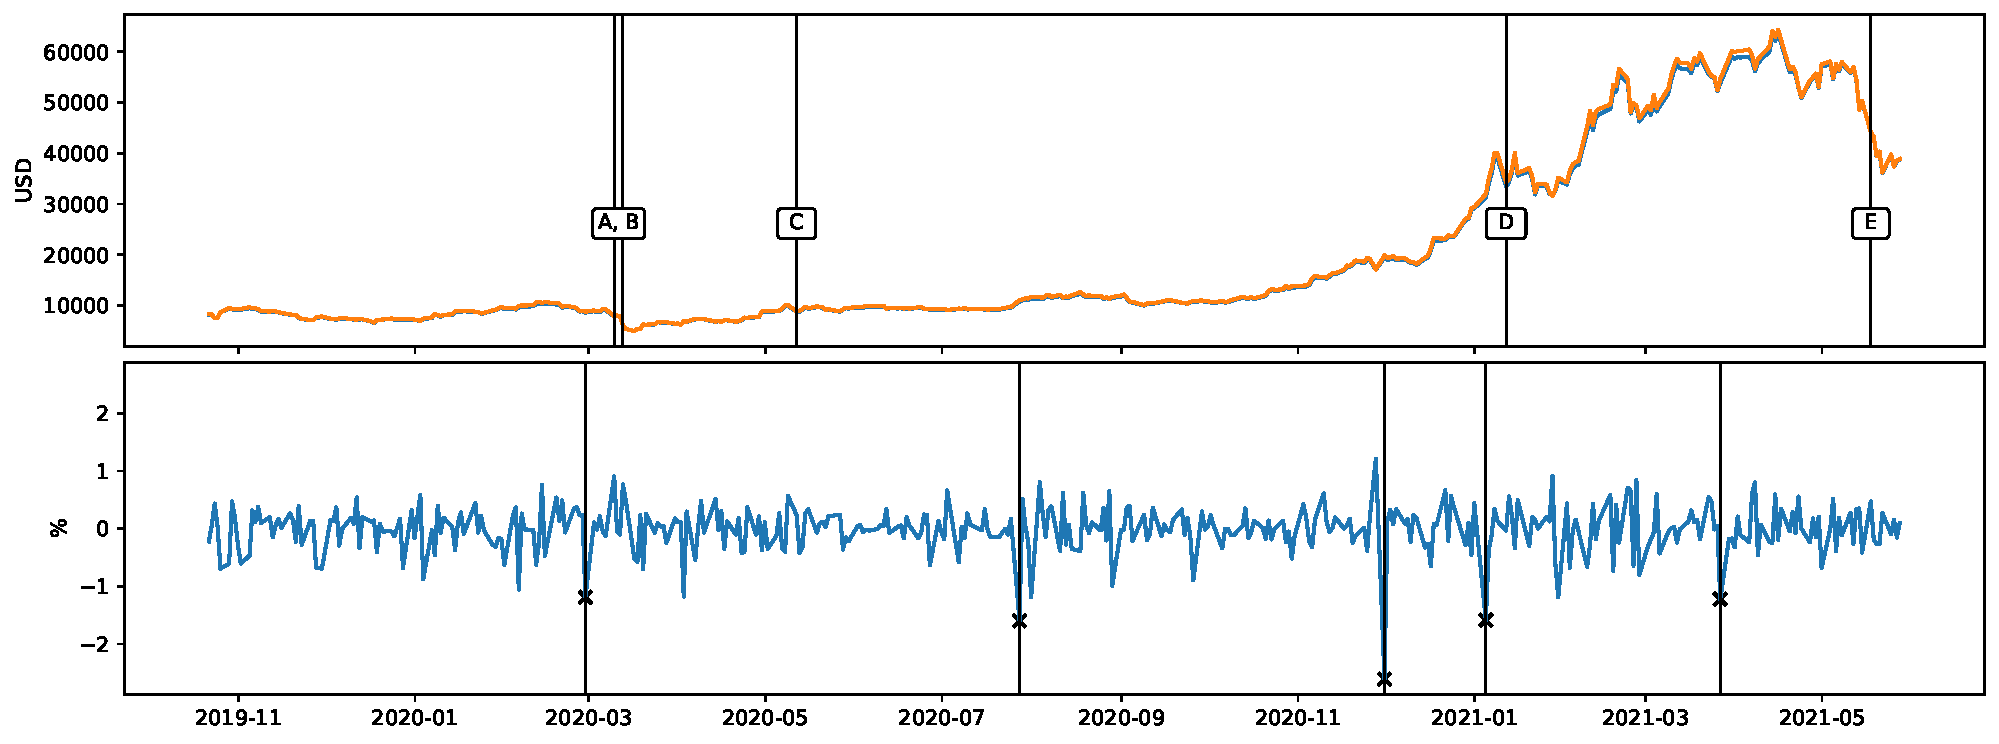
\includegraphics[width=\textwidth]{_pics/BTC_price.pdf}
  \caption{Out-of-sample BTC and BTCF price. The first panel presents the price of BTC in blue line and that of BTCF in orange line.
  The black vertical lines with capital letter labels indicate the five most negative daily return of BTC in the out-of-sample data.
  The second panel presents the difference between the daily log return of BTC and BTCF $r_s - r_f$.
  The black vertical lines with lowercase letter label indicate the five most negative difference.
  The crosses helps us better locate the level the difference.
  \href{http://www.quantlet.com/}{\includegraphics[height=\baselineskip]{_pics/qletlogo_tr.png}} }
\label{fig:BTC_price}
\end{figure}

\begin{figure}[t]
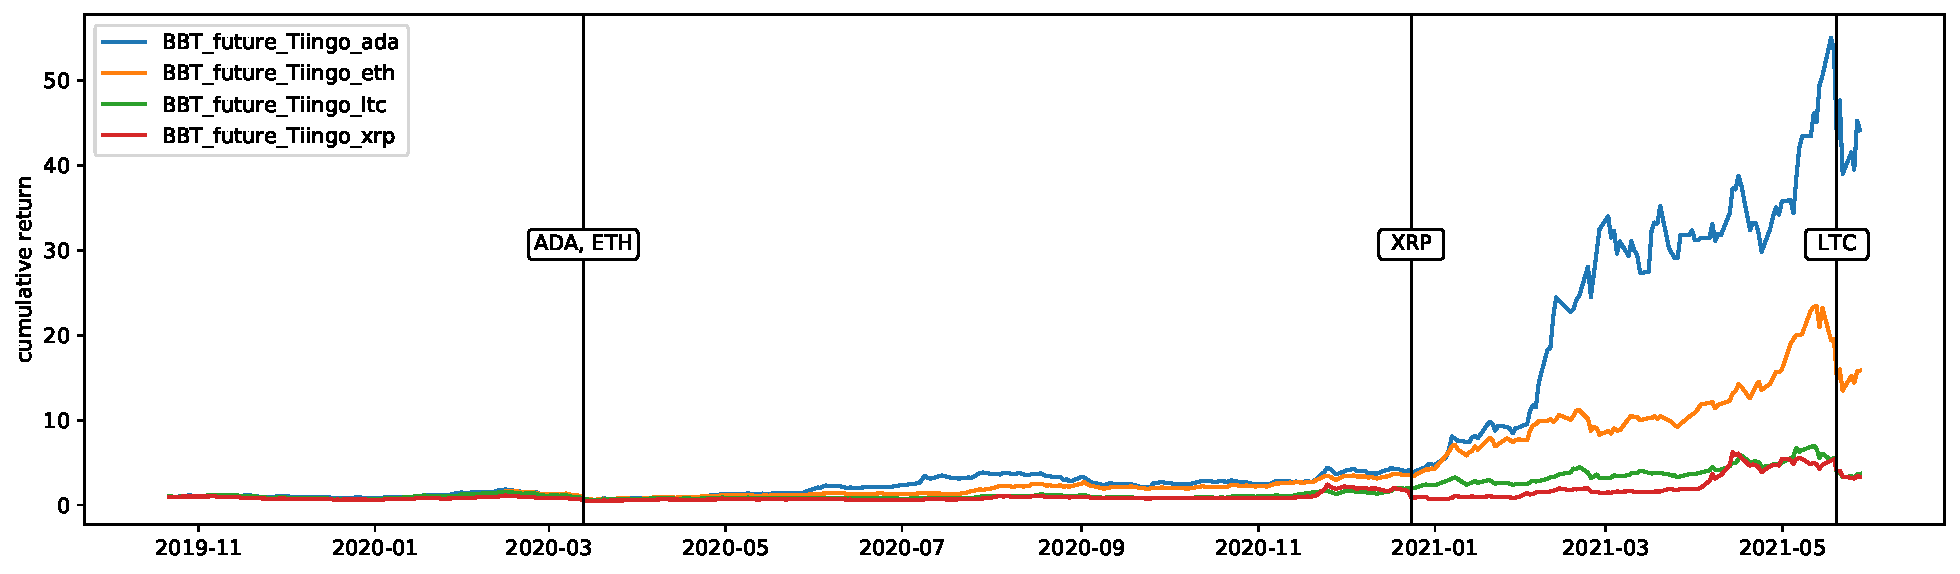
\includegraphics[width=\textwidth]{_pics/individualCoins_price.pdf}
  \caption{Out-of-sample cumulative return of individual cyptos.
  The black vertical lines indicate the most negative daily return of cryptos indicated by the labels.
  \href{http://www.quantlet.com/}{\includegraphics[height=\baselineskip]{_pics/qletlogo_tr.png}} }
\label{fig:individualCoins_price}
\end{figure}

\begin{figure}[t]
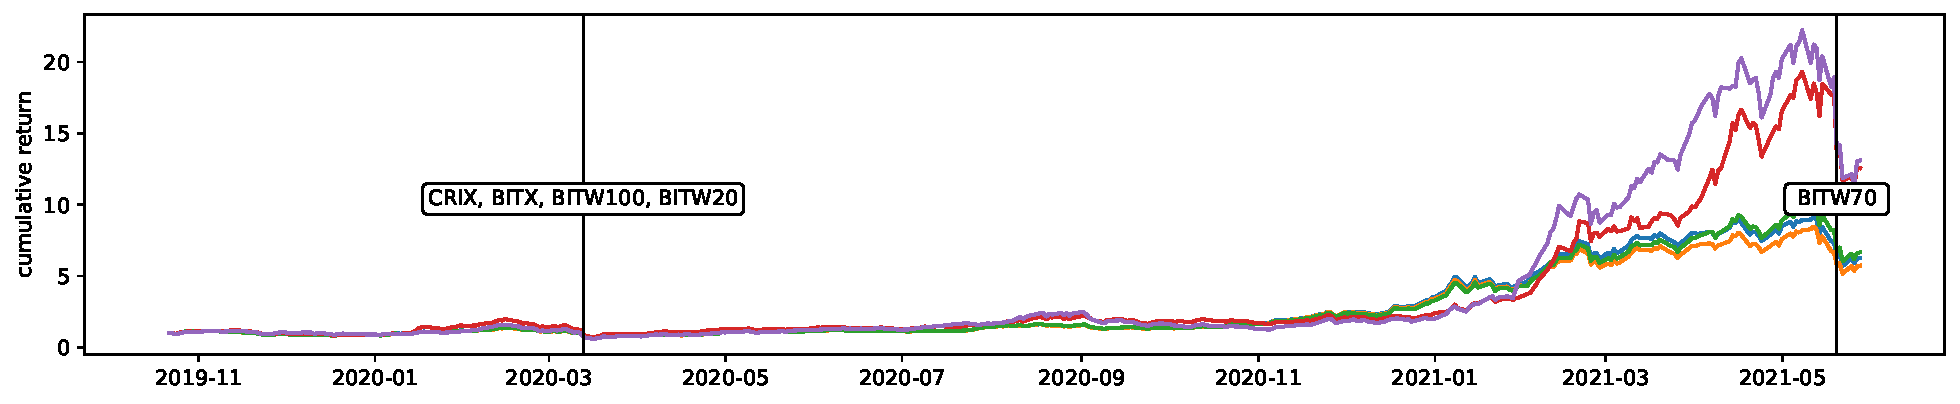
\includegraphics[width=\textwidth]{_pics/index_price.pdf}
  \caption{Out-of-sample cumulative return of crypto indices.
  The black vertical lines indicate the most negative daily return of indices indicated by the labels.
  \href{http://www.quantlet.com/}{\includegraphics[height=\baselineskip]{_pics/qletlogo_tr.png}} }
\label{fig:index_price}
\end{figure}

\newpage